%----------
\chapter{Makefiles}

	Es ist nicht m�glich, eine mit \textit{STORM} geschriebene Applikation mit Visual Studio
	in einem Schritt zu erstellen. Das Problem liegt beim CustomTool von CodeSmith. Zuerst
	wird aus den abstrakten Klassen eine DLL gebildet. Diese wird von CodeSmith verwendet
	um den Code zu generieren. Danach sollte die DLL mit dem neu dazugekommenen Code neu
	erzeugt werden. Dies ist jedoch erst nach einem Neustart von Visual Studio m�glich, 
	da die DLL durch das CodeSmith CustomTool blockiert wird.
	
	\section{L�sungsansatz}
	
		Mit Makefiles hat man die M�glichkeit die Applikation oder Libraries in einem Schritt 
		ohne das Aufstarten einer IDE zu erstellen. �nderungen in ben�tigten Dateien und 
		Abh�ngigkeiten werden automatisch erkannt.
		
		Wir haben zwei unabh�ngige Makefiles erstellt. Das eine �bernimmt das Bilden der 
		\textit{STORM} DLL. Damit ist es ebenfalls m�glich die DLL zu signieren und im GAC zu 
		registrieren.
		
		Mit dem zweiten Makefile ist es m�glich ein Assembly aus den abstrakten Klassen zu bilden, 
		daraus den ben�tigten Code zu generieren und dann die ganze HsrOrderApp Applikation zu 
		kompilieren. Das ganze geschieht mit einem einzigen Befehl.
		
	\section{Storm DLL}

		Das Makefile f�r die \textit{STORM} Library kann wie folgt ausgef�hrt werden:		
		\begin{Verbatim}
nmake [clean] [keys] [build] [install] [uninstall]
		\end{Verbatim}

		\begin{tabbing}
		  uninstall: \= \kill
			clean:     \> L�scht alle generierten Dateien aus dem Verzeichnis.\\
			keys:      \> Generiert ein Keypair.\\
			build:     \> Kompiliert und signiert den Code.\\
			install:   \> Registriert das Assembly im GAC.\\
			uninstall: \> Entfernt das Assembly aus dem GAC.\\
		\end{tabbing}

		In der Abbildung \ref{fig:analysisMakefilesStorm} sind die Abh�ngigkeiten der verschiedenen
		Schritte aufgezeigt. Wird zum Beispiel der Befehl \verb~install~ ausgef�hrt, wird auch �berpr�ft
		ob das Keypair vorliegt und die Storm.dll mit den aktuellsten Source Dateien kompiliert wurde.
		
		\begin{figure}[htb]
			\begin{center}
				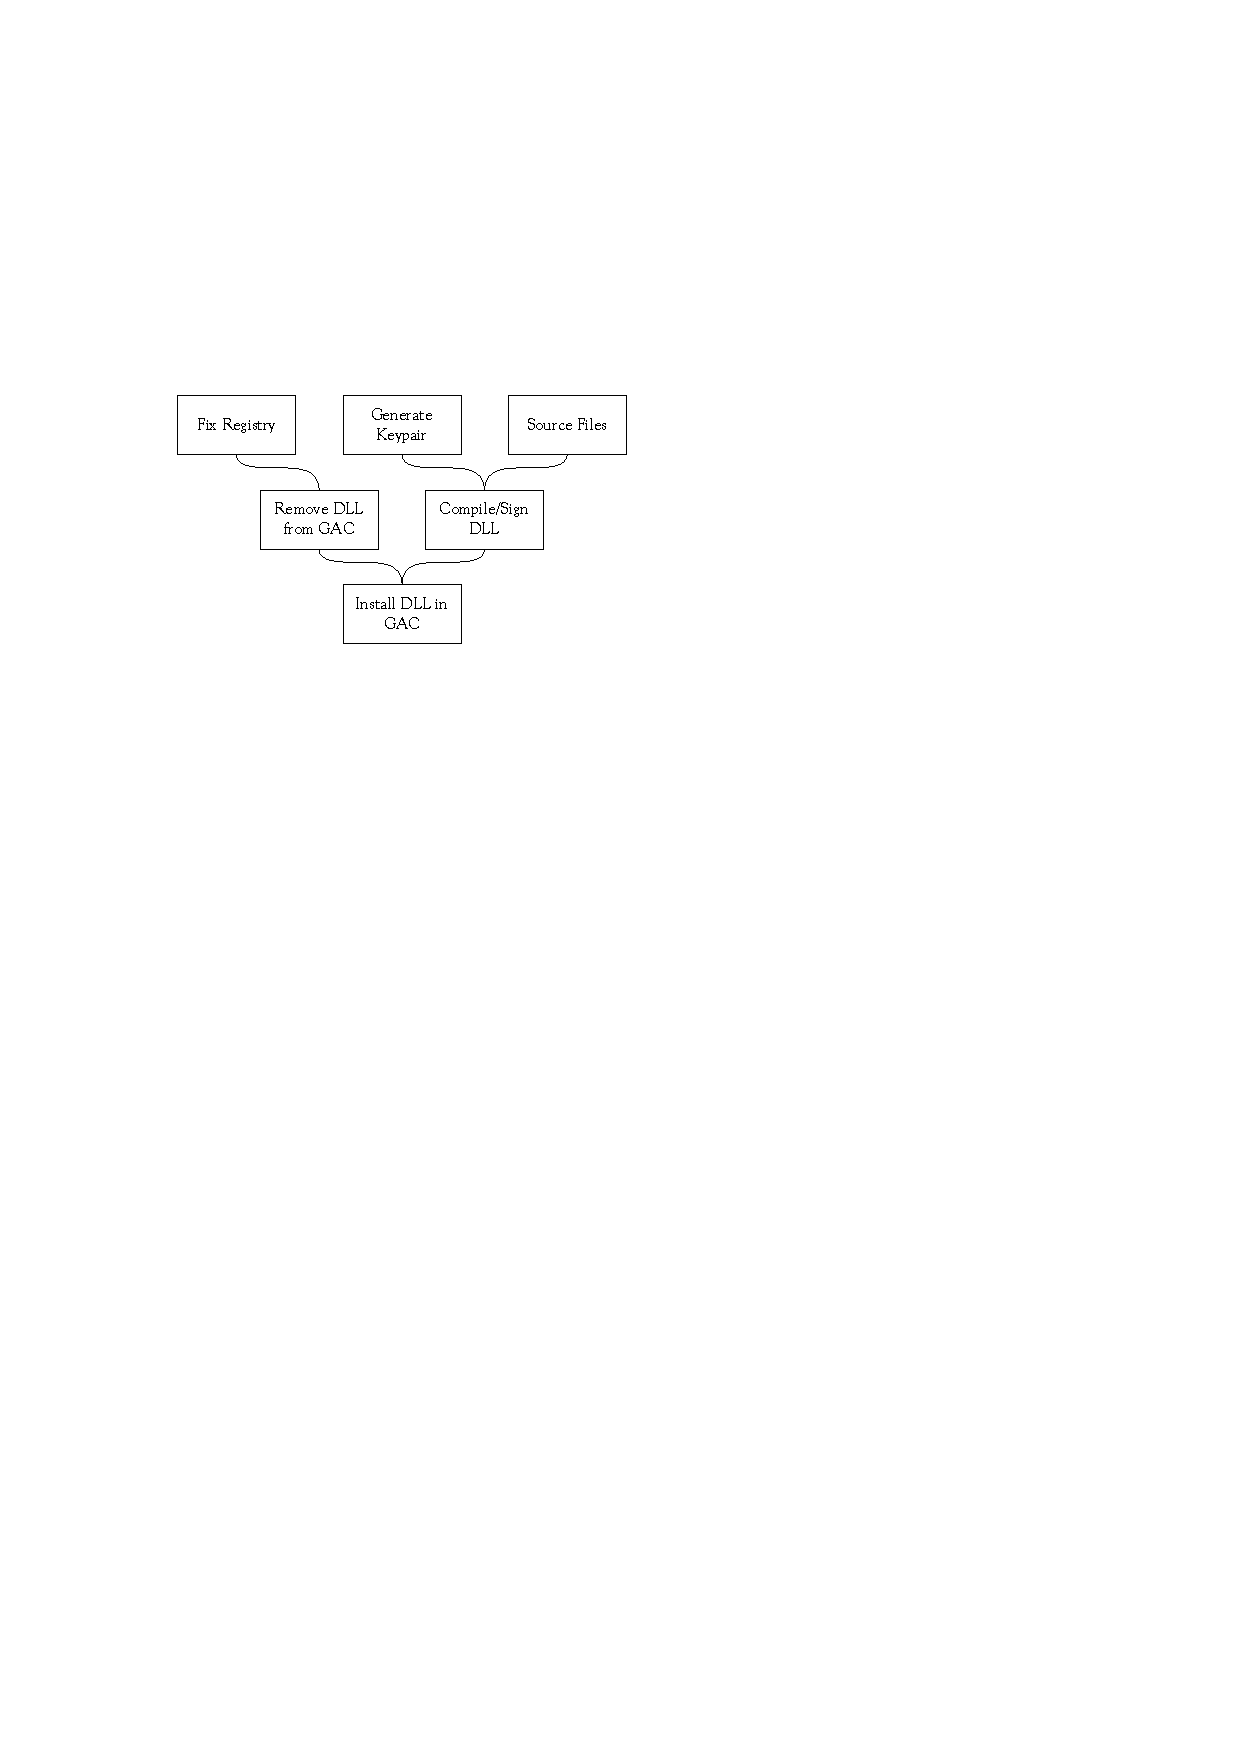
\includegraphics{./files/inc/figures/analysisMakefilesStorm}
				\caption{\label{fig:analysisMakefilesStorm} Storm Makefile}
			\end{center}
		\end{figure}

		Auf einigen Windows Installationen gibt es einen fehlerhaften Registry Eintrag, der wahrscheinlich 
		von einem Windows-Update stammt. Dieser verhindert, dass Assemblies aus dem GAC entfernt werden 
		k�nnen. Das Makefile l�scht diesen fehlerhaften Eintrag, bevor es versucht die DLL aus dem GAC zu 
		entfernen. Der Eintrag ist der Folgende:
		\begin{Verbatim}
[HKEY_LOCAL_MACHINE\SOFTWARE\Classes\Installer\Assemblies\Global]
@="..."
		\end{Verbatim}

\section{HsrOrderApp}
		
		Das Makefile f�r die HsrOrderApp kann wie folgt ausgef�hrt werden:		
		\begin{Verbatim}
nmake [clean] [impl] [mapper] [testapp] [run]
		\end{Verbatim}
		
		\begin{tabbing}
			testapp: \= \kill
			clean:   \> L�scht alle generierten Dateien aus dem Verzeichnis.\\
			impl:    \> Generiert mit Hilfe von CodeSmith die Implementations-Klassen\\
			         \> der Business-Objekte.\\
			mapper:  \> Generiert mit Hilfe von CodeSmith die Mapper-Klassen.\\
			testapp: \> Kompiliert die Applikation.\\
			run:     \> F�hrt die Applikation aus.\\
		\end{tabbing}
		
		Die Abbildung \ref{fig:analysisMakefilesOrderApp} zeigt die Abh�ngigkeiten beim bilden der 
		HsrOrderApp. Die Generierung von Domain Object Implementierungen und Mapper Klassen wurde 
		aufgeteilt, damit bei einer �nderung der Templates nur die betroffenen Dateien neu generiert 
		werden m�ssen. In der Abbildung wurde auf diese Aufteilung verzichtet.
		
		\begin{figure}[htb]
			\begin{center}
				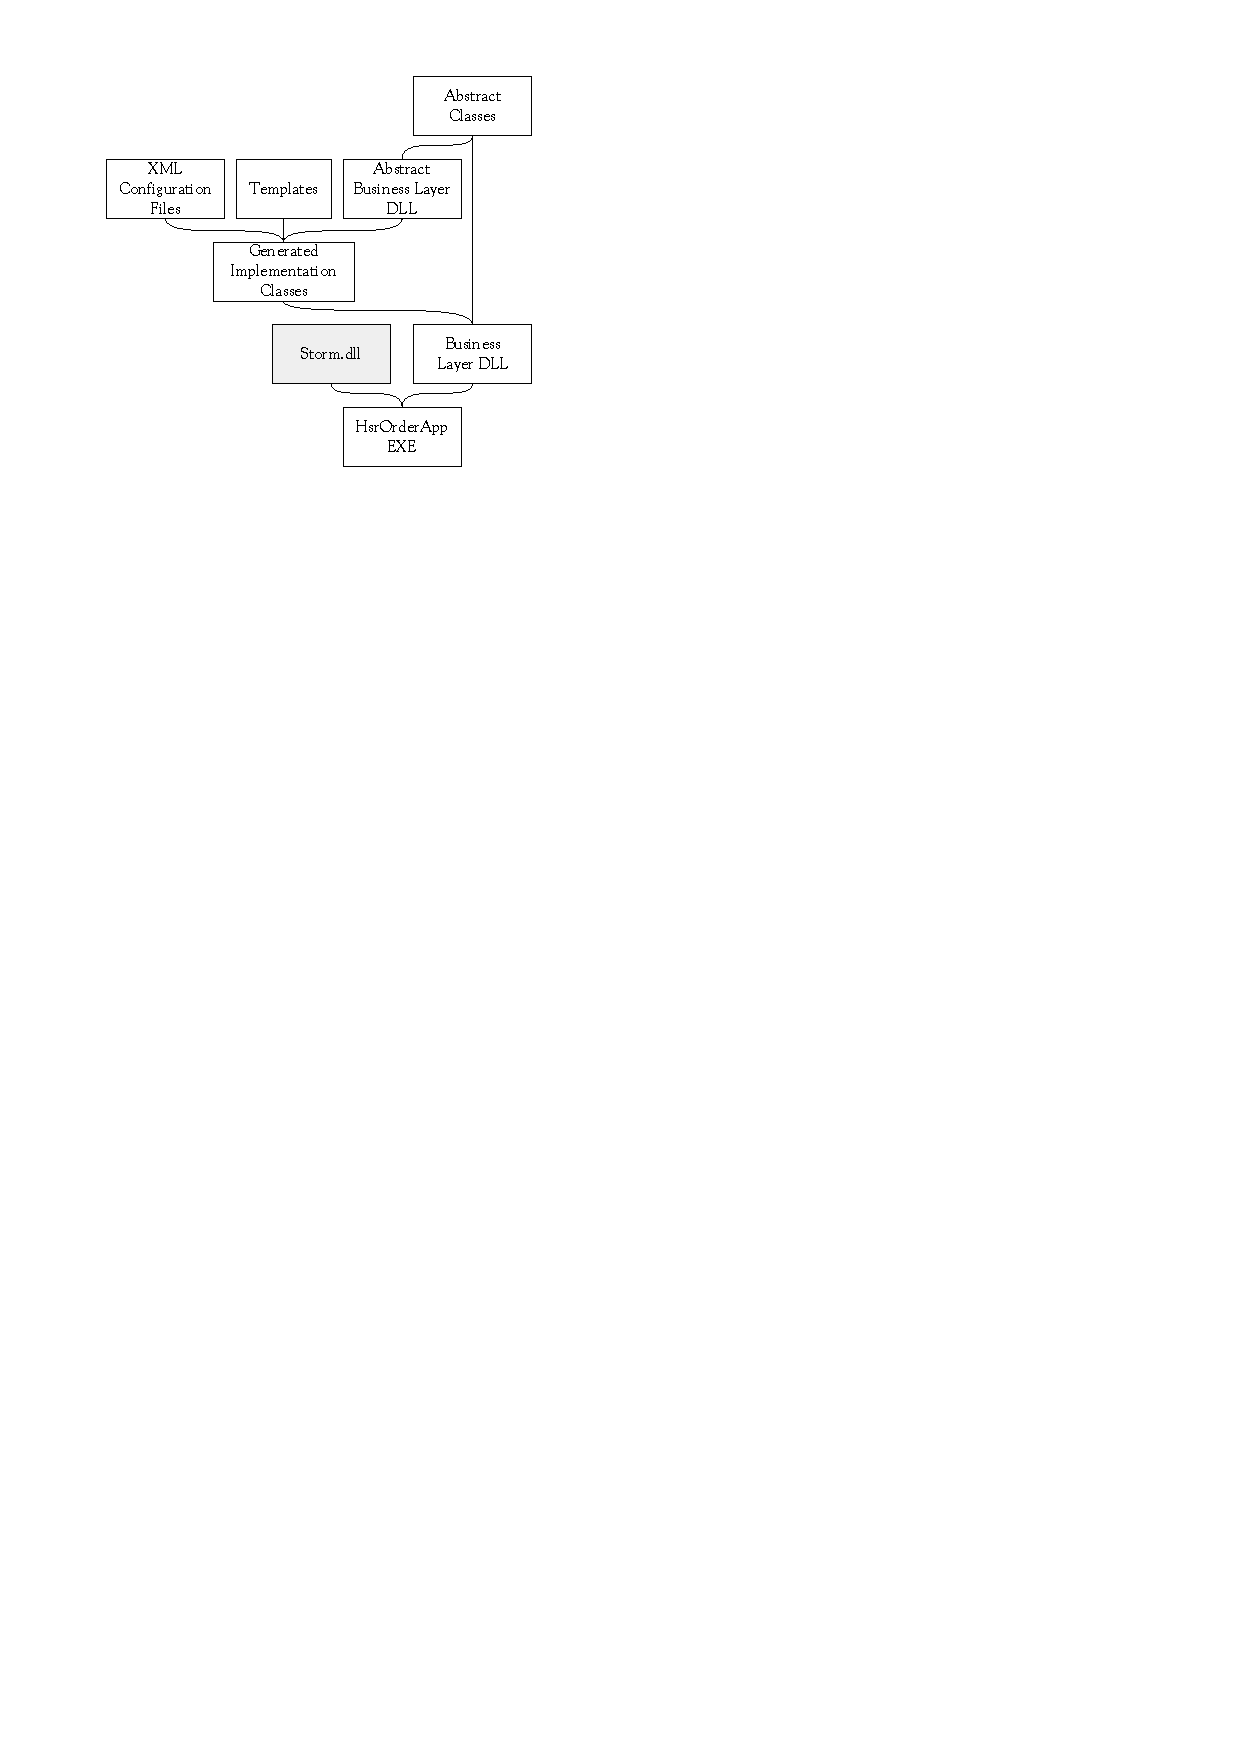
\includegraphics{./files/inc/figures/analysisMakefilesOrderApp}
				\caption{\label{fig:analysisMakefilesOrderApp} HsrOrderApp Makefile}
			\end{center}
		\end{figure}

		Die Datei Storm.dll wird vorausgesetzt und wird nicht automatisch erstellt.

	\section{Erkenntnisse}
		Den Build Prozess mit Makefiles zu automatisieren w�re eine sch�ne L�sung, den Code 
		auch ohne Visual Studio zu kompilieren. Ausserdem k�nnen andere Aufgaben wie Code 
		Generierung, Keypair erstellen, Code signieren und DLL im GAC registrieren im Build 
		Prozess eingebunden werden.
		
		Hier hat uns jedoch CodeSmith einen Strich durch die Rechnung gemacht. Denn aus 
		unerkl�rlichen Gr�nden, wird die DLL im GAC, w�hrend der Code Generierung, nicht 
		gefunden. Wir sind daher gezwungen unsere DLL ins Programm Verzeichnis von CodeSmith 
		zu kopieren, was alles andere als sch�n ist.
